Codeigniter adalah sebuah framework untuk web yang dibuat dalam format PHP. Format yang dibuat ini selanjutnya dapat digunakan untu membuat sistem aplikasi web yang kompleks. Codeigniter dapat mempercepat proses pembuatan web, karena semua class dan modul yang dibutuhkan sudah ada dan programmer hanya tinggal menggunakannya kembali pada aplikasi web yang akan dibuat \cite{prabowo2015website}.

\section{Tutorial Install CodeIgniter 3}
    \begin{enumerate}
        \item Pertama download Framework CodeIgniter di \textbf{\textit{https://www.codeigniter.com/}}
        
	    \item Setelah mengunduh file CodeIgniter 3, ekstrak file tersebut menggunakan WinRAR atau 7Zip kedalam folder htdocs jika kamu menggunakan XAMPP atau \textit{/var/www/html}. jika kamu menggunakan Apache2 Standalone, setelah itu ubahlan nama foldernya menjadi namaapplikasi.
	    
	    \item Sekarang silahkan Kamu coba akses URL \textbf{\textit{http://localhost/ namaaplikasi/}} melalui browser Kamu, akan langsung ditampilkan halaman awal Codeigniter yang berarti Instalasi telah berhasil.
		\begin{figure}[!htbp]
    		\centering
    		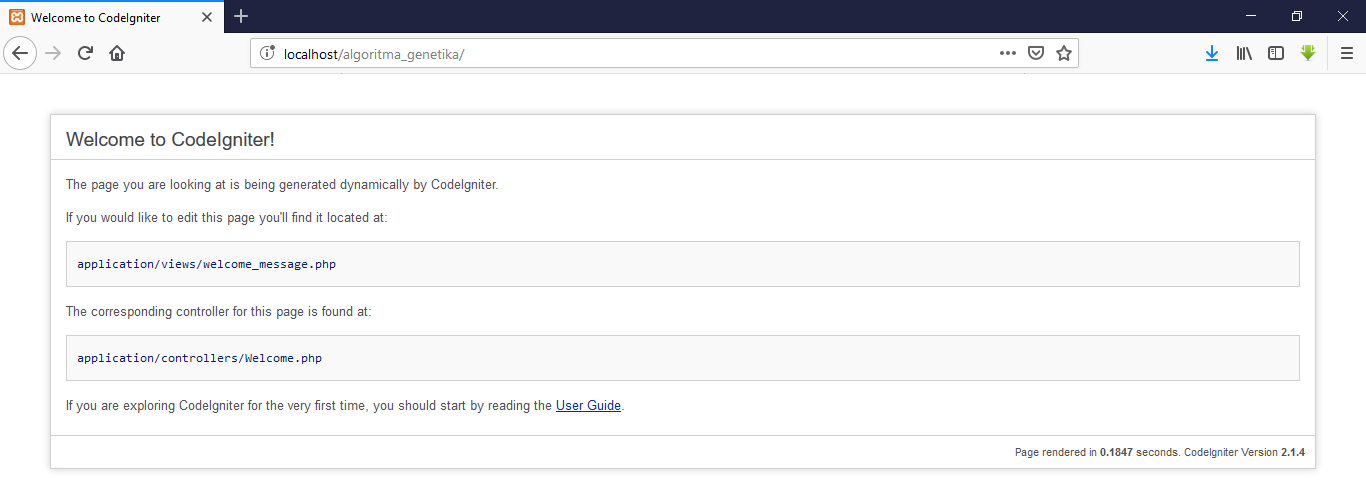
\includegraphics[width=0.5\textwidth]{figures/CodeIgniter1.PNG}
    		\label{Xampp2}
		\end{figure}
    \end{enumerate}
    
\section{Struktur CodeIginter}
\begin{enumerate}
    \item Folder \textbf{Application}, merupakan folder yang pada dasarnya menyimpan aplikasi yang sedang kita buat
    \item Folder \textbf{Cache}, merupakan folder yang menyimpan semua cache yang dibuat oleh cache library
    \item Folder \textbf{Config}, merupakan folder yang menyimpan informasi mengenai konfigurasi aplikasi seperti autoload, database, routes dan lainnya.
    \item Folder \textbf{Controller}, merupakan folder menyimpan controller - controller aplikasi yang dapat digunakan untuk menyusun aktivitas program .
    \item Folder \textbf{Core}, adalah folder untuk memperluas class class inti codeigniter.
    \item Folder \textbf{Helpers}, merupakan folder untuk menyimpan helpers.
    \item Folder \textbf{Hooks}, merupakan folder untuk menyimpan hooks untuk mengubah alur fungsi dari core Codeigniter
    \item Folder \textbf{Language}, merupakan folder untuk menyimpan bahasa - bahasa yang akan digunakan.
    \item Folder \textbf{Libraries}, merupakan folder untuk menyimpan library.
    \item Folder \textbf{Logs}, merupakan folder untuk menyimpan semua error log apabila error log diaktifkan.
    \item Folder \textbf{Models}, merupakan folder untuk menyimpan models yang akan mendefinisikan tabel dari database yang dapat kita gunakan oleh Controller yang kita buat untuk mengakses database.
    \item Folder \textbf{Third-party}, merupakan folder untuk menyimpan fungsi fungsi tambahan dalam cara kerja codeigniter.
    \item Folder \textbf{Views}, merupakan folder untuk menyimpan tampilan dari aplikasi yang kita buat.
    \item Folder \textbf{System}, merupakan folder untuk menyimpan sistem inti dari Codeigniter.
\end{enumerate}

\section{Konfigurasi CodeIgniter 3}
Di dalam folder application/config/ terdapat berbagai macam file konfigurasi yang dapat kita atur sendiri nantinya.
\begin{enumerate}
    \item \textbf{autoload.php}, digunakan untuk menambahkan package, libraries, drivers, helper, atau custom config lainnya agar secara otomatis diload oleh codeigniter.
    \item \textbf{config.php}, digunakan untuk membuat pengaturan dasar untuk web app codeigniter anda, seperti base-url, index page, cookie, proxy dan lain lain.
    \item \textbf{constants.php}, digunakan untuk kita dapat membuat constant baru.
    \item \textbf{database.php}, digunakan untuk mengatur koneksi web app kita ke database.
    \item \textbf{doctypes.php}, sebagai tempat penyimpanan deklarasi dokumen Doctype.
    \item \textbf{foreign-chars.php}, sebagai tempat penyimpanan karakter karakter asing.
    \item \textbf{hooks.php}, digunakan untuk mendefine "hooks" untuk meng extends CI
    \item \textbf{memcached.php}, config yang memungkinkan kita mencache database, driver dan lain lain sehingga lebih efektif.
    \item \textbf{migration.php}, config yang memungkinkan kita melakukan database migration. Secara default dijadikan False.
    \item \textbf{mimes.php}, menyimpan array yang berisi tipe file untuk fungsi upload.
    \item \textbf{profiler.php}, digunakan untuk mengatur profiler yang berguna pada saat debugging.
    \item \textbf{routes.php}, digunakan untuk mengatur default controllerdan overide 404
    \item \textbf{smileys.php}, menyimpan array yang berisi smiley yang membantu helper emoticon.
    \item \textbf{user-agents.php}, menyimpan data user agent, yang membantu class User Agen untuk mengidentifikasi browser, platform, robotdan datamobile device
\end{enumerate}

Pada konfigurasi yang saya lakukan hanya melukakan konfigurasi pada file autoload.php, config.php, database.php dan routes.php. Berikut cara konfigurasinya:
\begin{enumerate}
    \item Autoload.php
		\begin{figure}[!htbp]
    		\centering
    		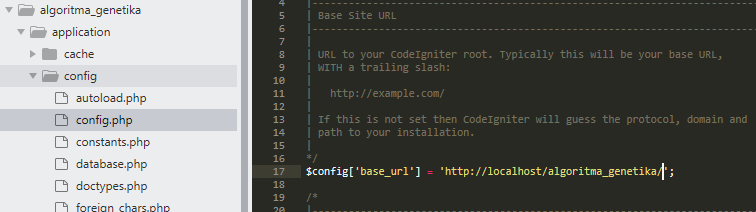
\includegraphics[width=0.5\textwidth]{figures/CodeIgniter2.PNG}
    		\label{CodeIgniter2}
		\end{figure}
		\par Pada file ini saya meng-input libraries untuk support framework CodeIgniter ini terhadap database, form-validation yang akan dibuat nantinya, pagination dan Session untuk mengaktifkan session pada CodeIgniter.
        Pada variable autoload helper saya meng-input url dan form semua di inputkan sesuai dengan kebutuhan pembuat aplikasi. Array tersebut akan di eksekusi secara automatis oleh CodeIgniter.

    \item Config.php
		\begin{figure}[!htbp]
    		\centering
    		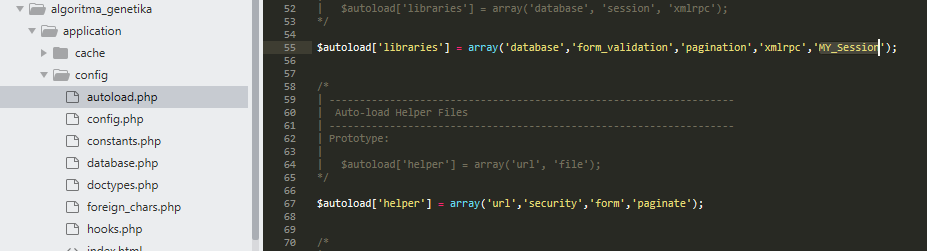
\includegraphics[width=0.5\textwidth]{figures/CodeIgniter3.PNG}
    		\label{CodeIgniter3}
		\end{figure}
        \par Pada config.php inputkan url utama aplikasi pada variable config base-url seperti pada gambar diatas.
        
    \item Database.php
		\begin{figure}[!htbp]
    		\centering
    		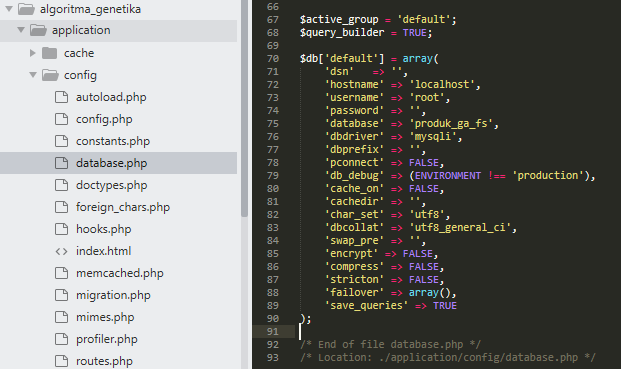
\includegraphics[width=0.6\textwidth]{figures/CodeIgniter4.PNG}
    		\label{CodeIgniter4}
		\end{figure}
		\par Pada database.php konfigurasi yang dilakukan untuk mengkoneksikan database yaitu MySQL dengan aplikasi web berbasis framework CodeIgniter. Dapat dilihat pada line 72, hostname yang diiniputkan sesuai dengan hostname yang dipakai, disini saya menginputkna localhost dengan username default yaitu root password dikosongkan karena pada Xampp saya tidak menggunakan password. Pada database line 75 inputkan nama database sesuai dengan nama database yang ada pada MySQL.
		
	\item Routes.php
		\begin{figure}[!htbp]
    		\centering
    		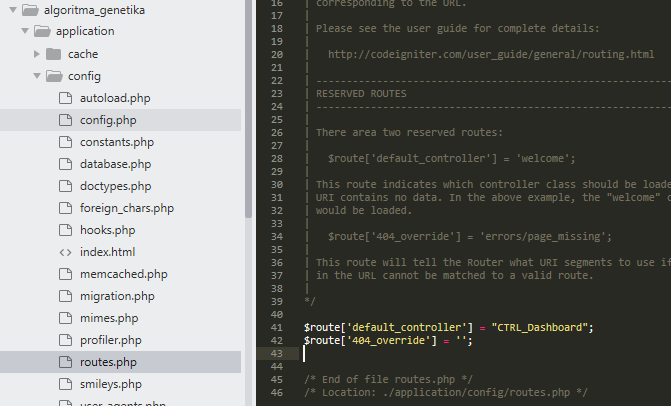
\includegraphics[width=0.7\textwidth]{figures/CodeIgniter5.PNG}
    		\label{CodeIgniter5}
		\end{figure}
		\par Pada file ini dilakukan konfigurasi dimana controller mana yang akan pertama di eksekusi ketika url dijalankan.
\end{enumerate}

\section{Konfigurasi Bootstrap dan Template CodeIgniter 3}
\section{MVC dan CRUD CodeIgniter 3}